\question{Câu 8}

Cho mạch khuếch đại như hình vẽ, mạch có $R_{in} = 400\,\text{k}\Omega$ và $V_{DD} = 5V$. $M_{1}$ và $M_{2}$ có $k_{n} = 200\,\mu \text{A/V}^{2}$, $V_{tn} = 0.6\,\text{V}$, $K_{p2} = 1\,\text{mA/V}^{2}$, $V_{TP2} = -0.6\,\text{V}$ và $V_{A1} = V_{A2} = \infty$, giả sử các tụ có giá trị rất lớn.

\begin{figure}[H]
	\centering
	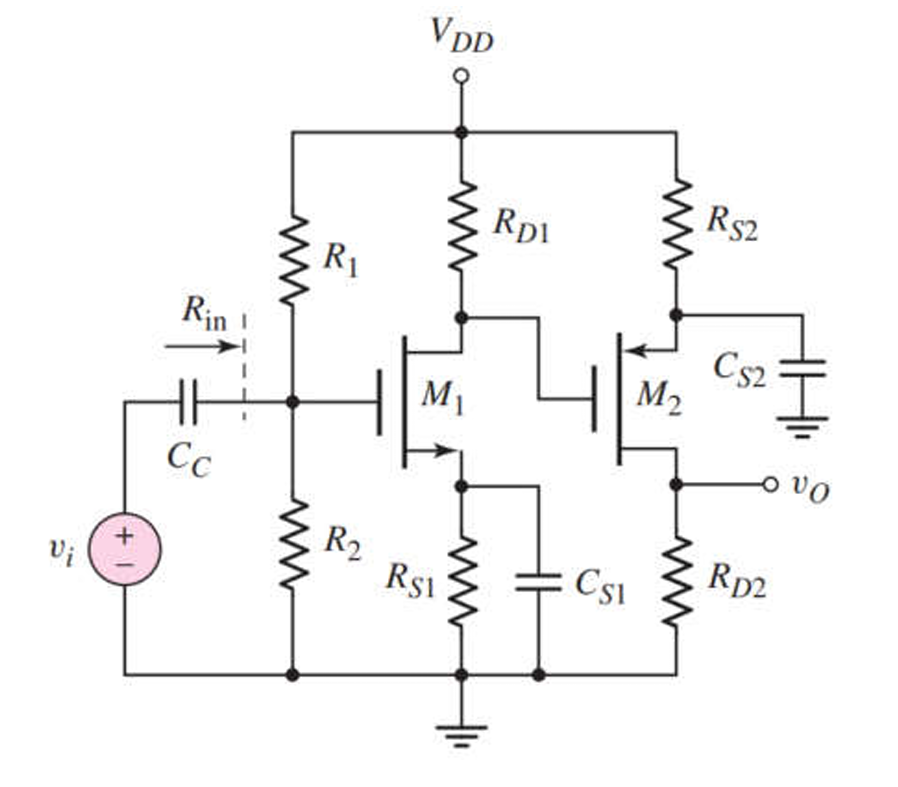
\includegraphics[width=.8\linewidth]{./my-chapters/my-images/Question8/debai.png}
\end{figure}

\answer{a}{Thiết kế mạch để $M_{1}$ có $Q_{1}(I_{DS1}=0.2\,\textsf{mA ,} V_{DS1} = 2\,\textsf{V})$, $M_{2}$ có $Q_{2}(I_{DS2}=0.5\,\textsf{mA ,} V_{SD2} = 3\,\textsf{V})$ và điện áp DC trên $R_{S1} = 0.6\,\textsf{V}$}

	$ R_{S1} = \dfrac{V_{RS1}}{I_{D1}} 
	= \dfrac{0.6}{0.2} 
	= 3\,k\Omega $ $\Rightarrow$ \finalresult{R_{S1} = 3\,\text{k}\Omega}.
	
	\( V_{DD} - V_{DS1} = I_{D1} (R_{D1} + R_{S1}) 
	\Rightarrow 5 - 2 = 0.2 (R_{D1} + 3k) \) $\Rightarrow$ \finalresult{R_{D1} = 12\,k\Omega}. 
	
	\( I_{DS1} = \dfrac{1}{2} k_n (V_{GS1} - V_{thn})^2 
	\Rightarrow 0.2 = \dfrac{1}{2} (200 \times 10^{-3}) (V_{GS1} - 0.6)^2 
	\Rightarrow V_{GS1} = 2.014\,\text{V} \)
	
	\( \dfrac{R_2}{R_1 + R_2} V_{CC} - V_{RS1} = V_{GS1} 
	\Rightarrow \dfrac{R_2}{R_1 + R_2} \cdot 5 - 0.6 = 2.014 
	\Rightarrow \dfrac{R_2}{R_1 + R_2} = 0.5228 \)
	
	\( \Rightarrow 0.9123 R_2 = R_1 \quad (1) \)
	
	Với \( R_{in} = R_1 // R_2 = 400\,k\Omega \quad (2) \)
	
	Từ (1) và (2) 
	
	\[\Rightarrow 
	\begin{cases}
		\finalresult{R_2 = 838.45\,k\Omega} \\
		\finalresult{R_1 = 764.9\,k\Omega}
	\end{cases}
	\]


	\( I_{SD2} = \dfrac{1}{2} k_p (V_{SG2} - |V_{thp}|)^2 
	\Rightarrow 0.5 = \dfrac{1}{2} (1) (V_{SG2} - 0.6)^2 
	\Rightarrow V_{SG2} = 1.6\,\text{V} \)
	
	\( V_{DD} - I_{D2} R_{S2} - (V_{DD} - I_{D1} R_{D1}) = 1.6 
	\Rightarrow I_{D1} R_{D1} - I_{D2} R_{S2} = 1.6 \)
	
	\( \Rightarrow 0.2 \times 12k - 0.5 R_{S2} = 1.6 \)
	
	$\Rightarrow $ \finalresult{R_{S2} = 2.4\,k\Omega}.

\answer{b}{Đặt $v_{s} = 2 \sin \left( \omega t \right) (\text{mV})$ vào mạch. Ngõ ra nối với tải $R_{L} = 1\,\text{k}\Omega$. Tìm $A_{v}$, $G_{v}$, $R_{in}$, $R_{out}$ của mạch.}

Từ câu a ta có mạch tổng quan như sau,

\begin{figure}[H]
	\centering
	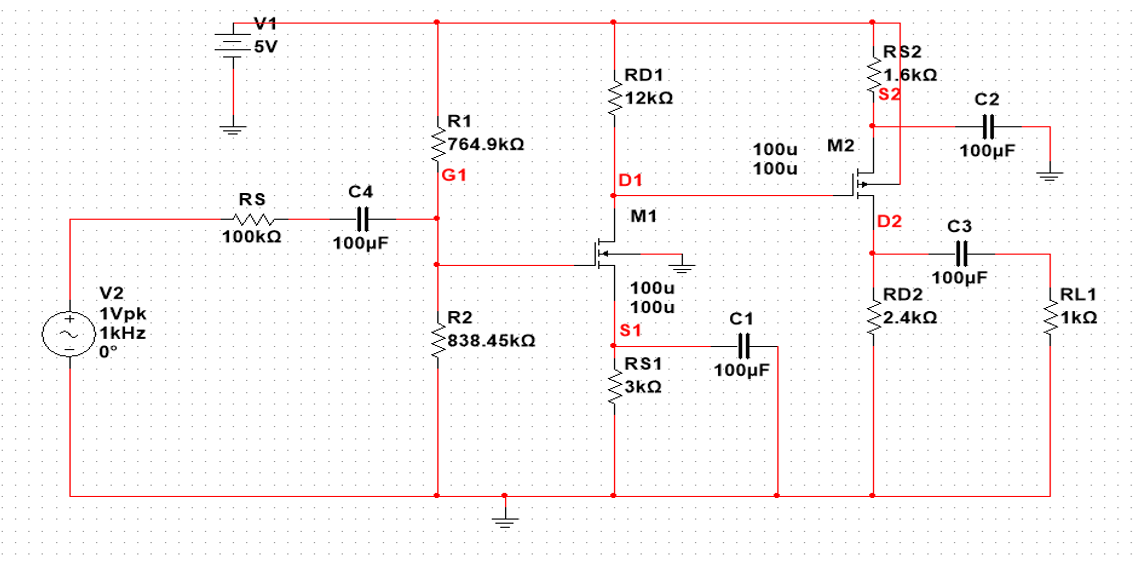
\includegraphics[width=.8\linewidth]{./my-chapters/my-images/Question8/b_tongquan.png}
\end{figure}

Ta xét hoạt động AC, với mạch tương đương như sau

\begin{figure}[H]
	\centering
	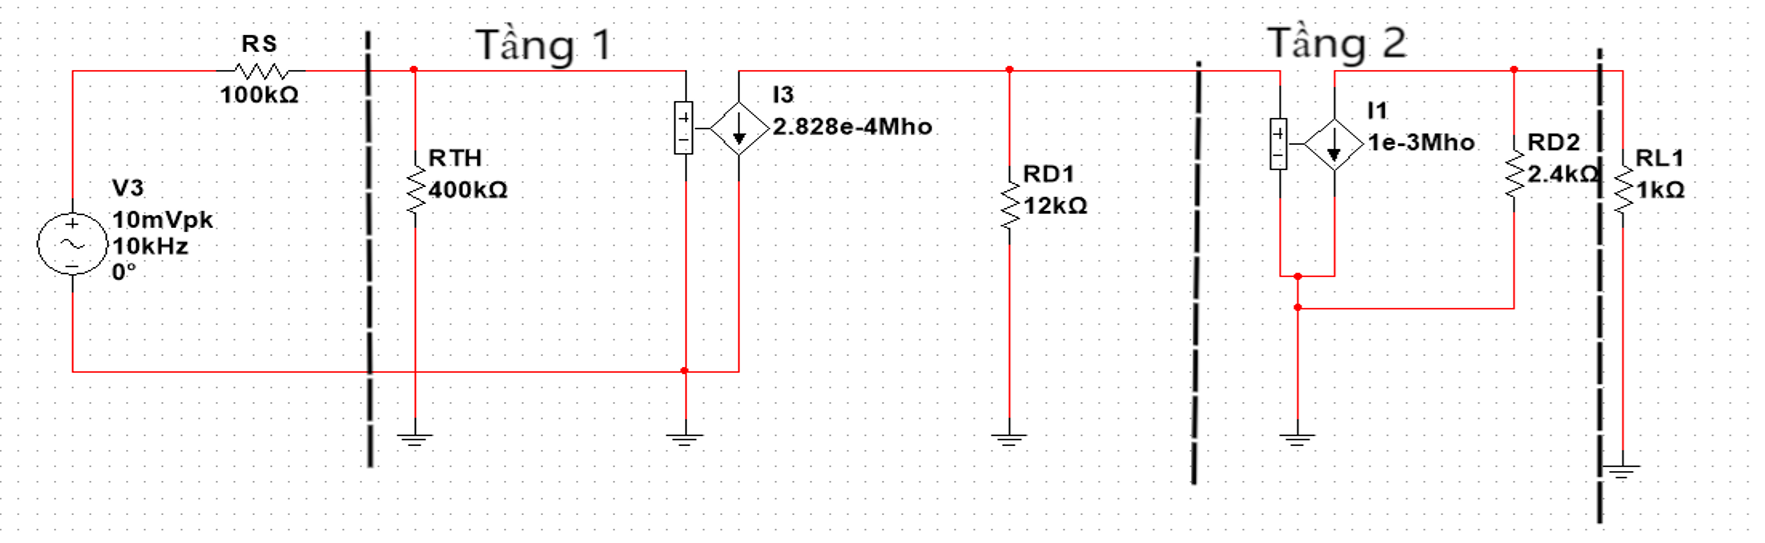
\includegraphics[width=.8\linewidth]{./my-chapters/my-images/Question8/b_mohinhtuongduong.png}
\end{figure}

\begin{itemize}[label=+, leftmargin=2cm]
	\item \( g_{m1} = k_n (V_{GS1} - V_{thn})
	= 200\times 10^{-6}\,(2.014-0.6)
	= 0.0002828\ \text{S}
	= 2.828\times 10^{-4}\ \text{S} \)
	\item \( g_{m2} = k_p (V_{SG2} - |V_{thp}|)
	= 1\times 10^{-3}\,(1.6-0.6)
	= 0.001\ \text{S} \)
\end{itemize}

\begin{itemize}[label=-]
	\item Tầng 1
	\begin{itemize}[label=+, leftmargin=2cm]
		\item \( R_{in1} = R_{TH} = 400\,k\Omega \)
		\item \( R_{out1} = R_{D1} = 12\,k\Omega \)
		\item \( A_{vo1} = -g_{m1} R_{D1}
		= -0.0002828 \times 12000
		= -3.3936 \ (\text{V/V})
		\approx -3.39\ (\text{V/V}) \)
	\end{itemize}
	
	\item Tầng 2
	\begin{itemize}[label=+, leftmargin=2cm]
		\item \( R_{in2} \to \infty \) (cổng)
		\item \( R_{out2} = R_{D2} = 2.4\,k\Omega \)
		\item \( A_{vo2} = -g_{m2} R_{D2}
		= -0.001 \times 2400
		= -2.4\ (\text{V/V}) \)
	\end{itemize}
	
	\item Toàn mạch
	\begin{itemize}[label=+, leftmargin=2cm]
		\item \finalresult{R_{in} = R_{in1} = 400\,k\Omega}
		
		\item \finalresult{R_{out} = R_{out2} = 2.4\,k\Omega}
		
		\item $	A_{vo} = A_{vo1} A_{vo2}\frac{R_{in2}}{R_{out1}+R_{in2}} = 8.136 (\text{V/V}).$
		
		$\Rightarrow$ \finalresult{A_{vo} = 8.136 (\text{V/V})}.
		
		\item $ A_{v} = A_{vo}\dfrac{R_{L}}{R_{out} + R_{L}} = 2.39 (\text{V/V})$
		
		$\Rightarrow$ \finalresult{A_{v} = 2.39 (\text{V/V})}.
		
		\item $G_{v} = A_{v} \dfrac{R_{in}}{R_{in} + R_{s}} = 1.91 (\text{V/V})$
		
		$\Rightarrow$ \finalresult{ G_{v} = 1.91(\text{V/V})}.
	\end{itemize}
	
	\item Kiểm tra kết quả
	
	\begin{figure}[H]
		\centering
		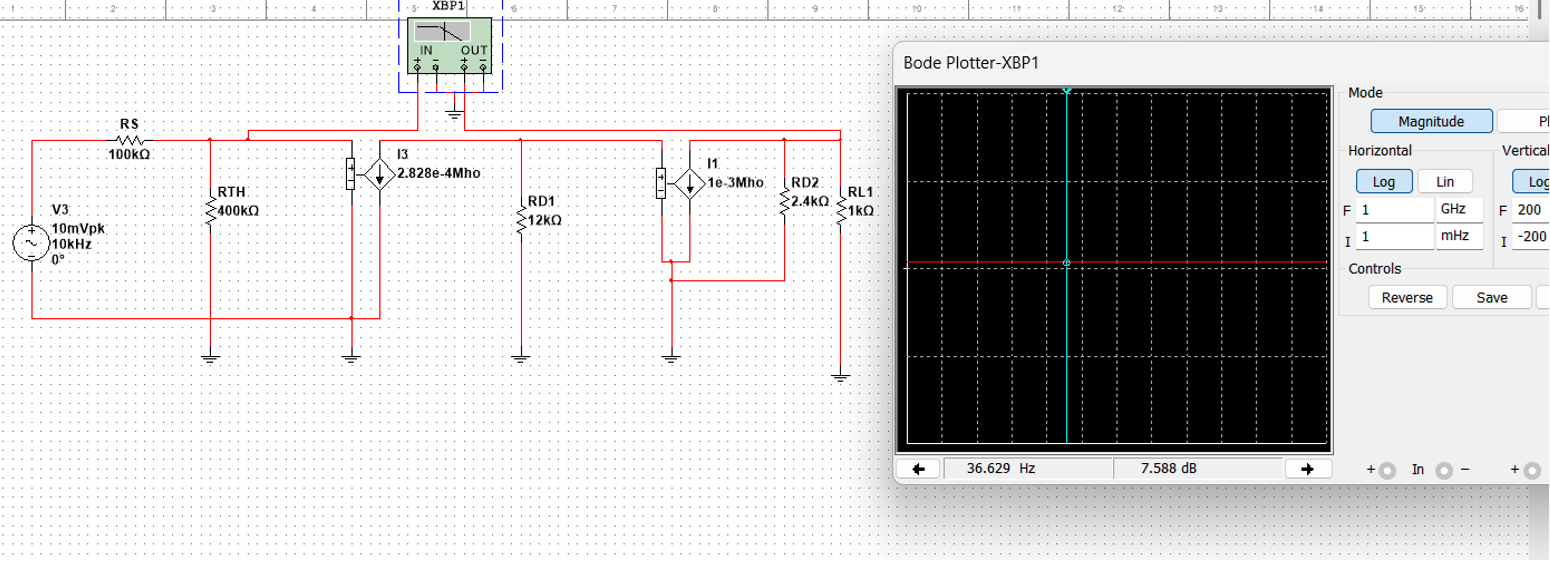
\includegraphics[width=.9\linewidth]{./my-chapters/my-images/Question8/b_av_tuongduong.png}
		\caption{Đo $|A_{v}| =7.558 db = 2.4 \,\textsf{V/V}$ (mô hình tương đương).}
	\end{figure}
	\begin{figure}[H]
		\centering
		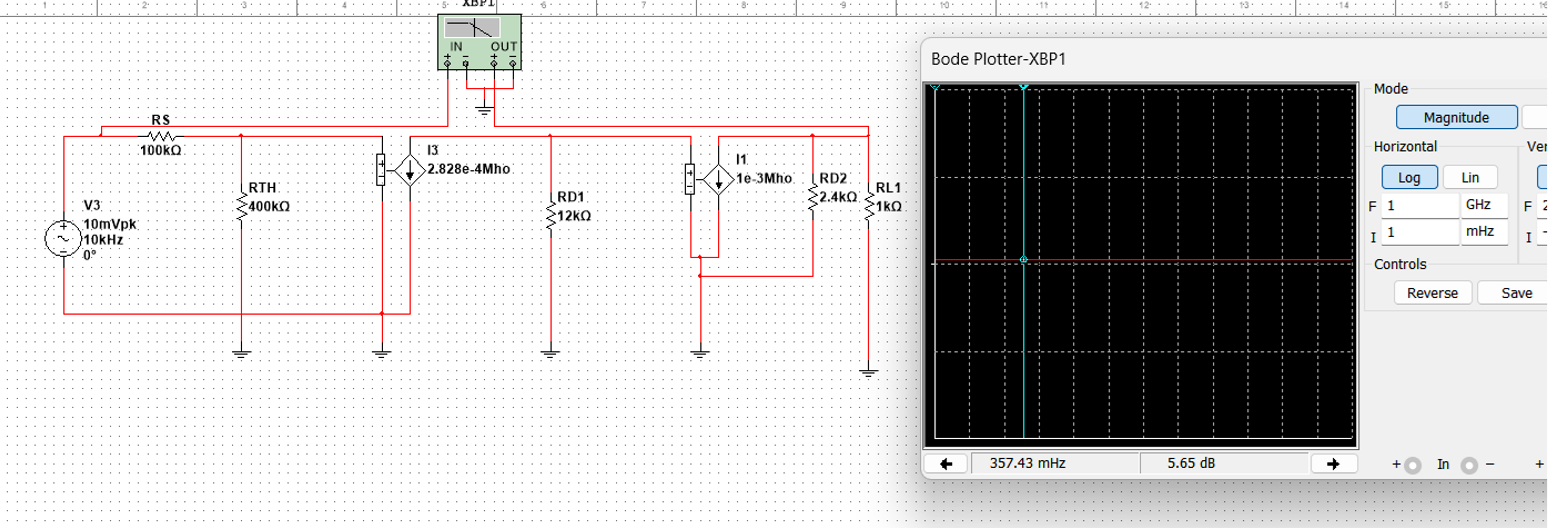
\includegraphics[width=.9\linewidth]{./my-chapters/my-images/Question8/b_gv_tuongduong.png}
		\caption{Đo $|G_{v}| = 5.65db = 1.91 \,\textsf{V/V}$ (mô hình tương đương).}
	\end{figure}
	\begin{figure}[H]
		\centering
		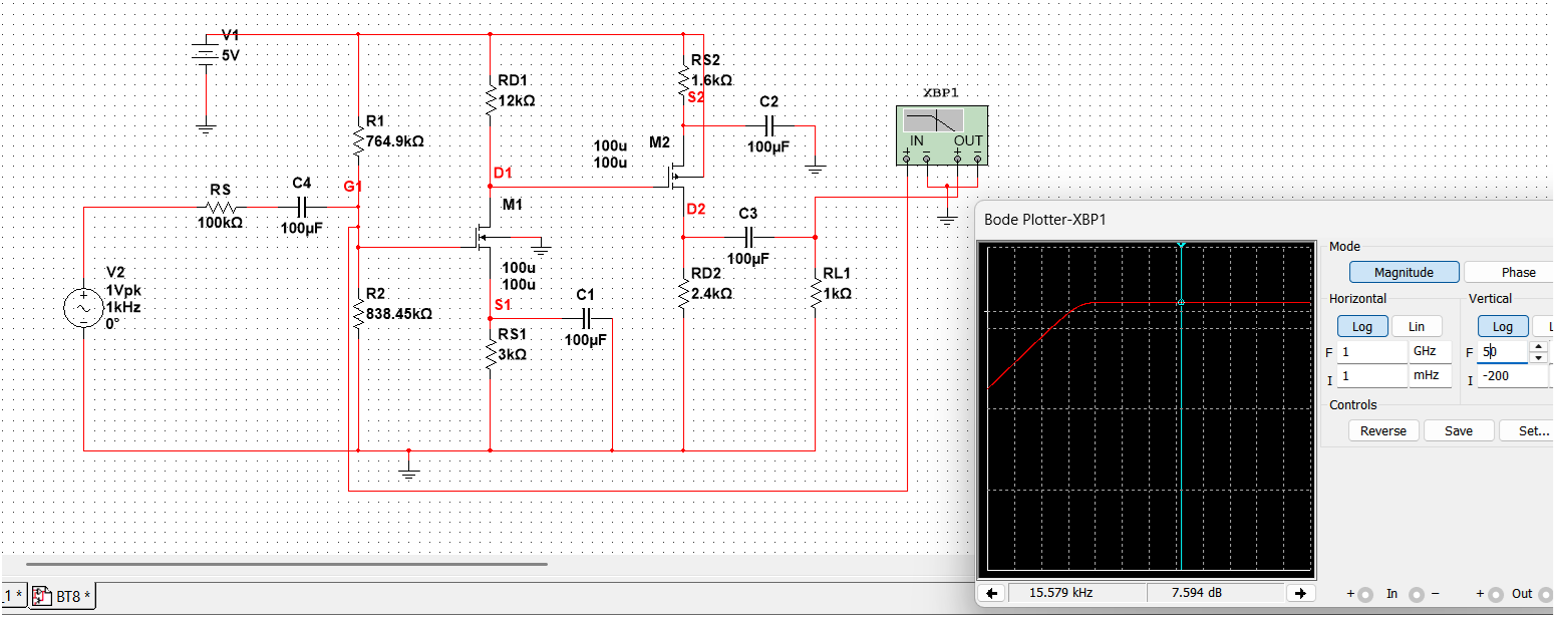
\includegraphics[width=.9\linewidth]{./my-chapters/my-images/Question8/b_av_toanmach.png}
		\caption{Đo $|A_{v}| = 7.594db = 2.4 \,\textsf{V/V}$ (mô hình toàn mạch).}
	\end{figure}
	\begin{figure}[H]
		\centering
		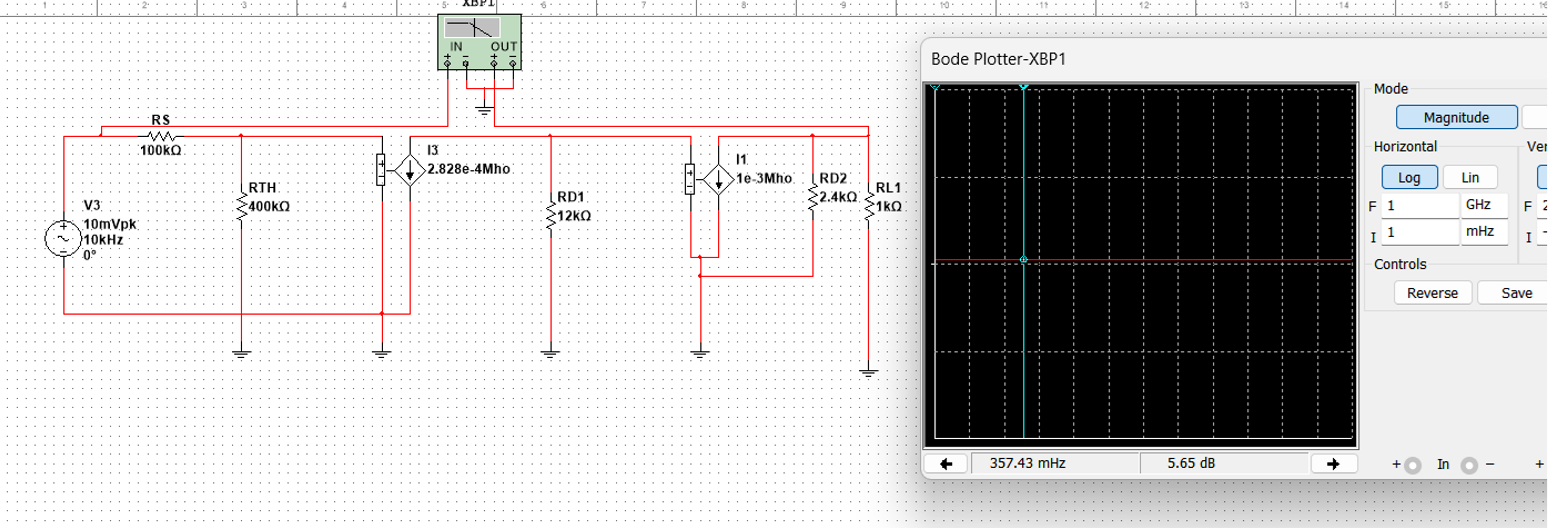
\includegraphics[width=.9\linewidth]{./my-chapters/my-images/Question8/b_gv_tuongduong.png}
		\caption{Đo $|G_{v}| = 5.655 db = 1.92 \,\textsf{V/V}$ (mô hình toàn mạch).}
	\end{figure}
\end{itemize}

\answer{c}{Vẽ ngõ ra $v_{o}$}

\begin{figure}[H]
	\centering
	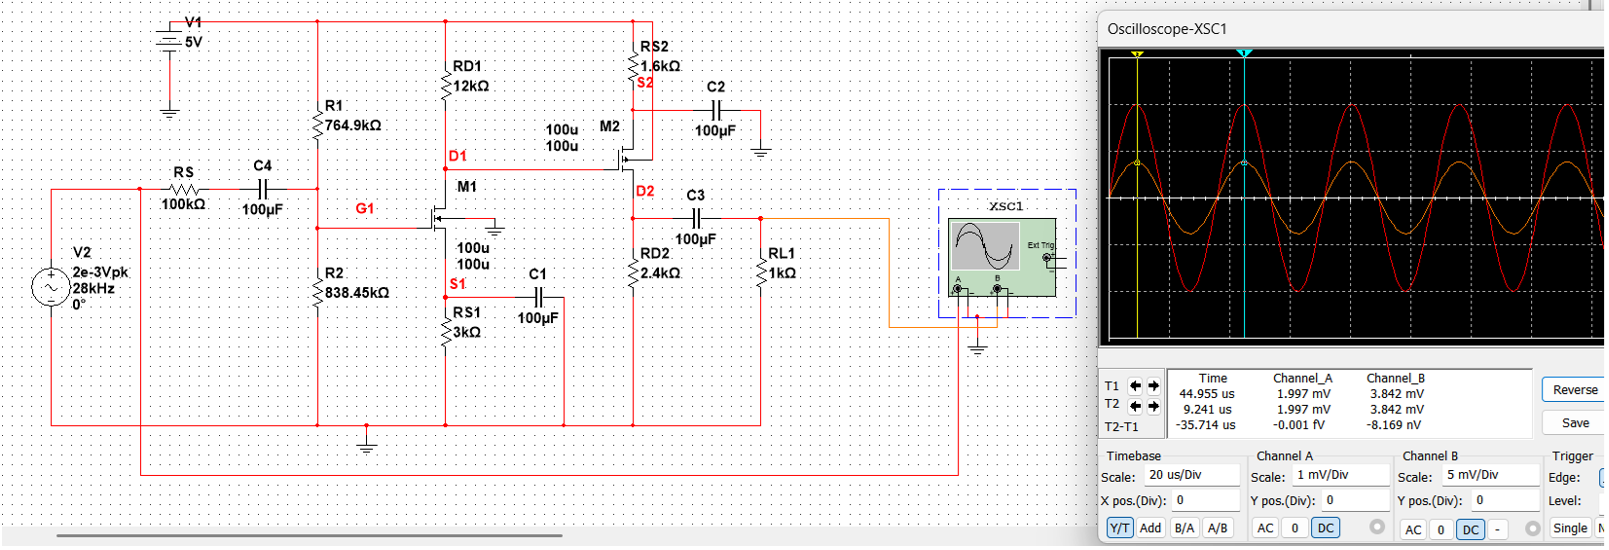
\includegraphics[width=\linewidth]{./my-chapters/my-images/Question8/c_test.png}
	\caption{$V_{psig} = 2\,\textsf{mV}$, $V_{pL} = 3.842 \,\textsf{mV}$, $G_{v} = 1.921 \,\textsf{V/V}$.}
\end{figure}

\answer{d}{Lựa chọn các tụ $C_{C}$, $C_{S2}$ để mạch có $f_{L}=100\,\textsf{Hz}$.}

\begin{itemize}[label=-]
	\item Xét tụ $C_4$: 
	\[
	\tau_4 = R_5 + R_{TH} = 100k + 400k = 500k 
	\quad\Rightarrow\quad 
	f_4 = \frac{1}{2\pi\tau_4 C_4}
	\]
	\item Xét tụ $C_1$: 
	\[
	\tau_1 = R_{S1} = 3k 
	\quad\Rightarrow\quad 
	f_1 = \frac{1}{2\pi\tau_1 C_1}
	\]
	\item Xét tụ $C_2$: 
	\[
	\tau_2 = R_{S2} = 1.6k 
	\quad\Rightarrow\quad 
	f_2 = \frac{1}{2\pi\tau_2 C_2}
	\]
	\item Xét tụ $C_3$: 
	\[
	\tau_3 = R_{D2} + R_L = 2.4k + 1k = 3.4k 
	\quad\Rightarrow\quad 
	f_3 = \frac{1}{2\pi\tau_3 C_3}
	\]
\end{itemize}

\noindent Ta có: 
\[
\tau_2 < \tau_1 < \tau_3 < \tau_4 
\quad\Rightarrow\quad 
\text{Để tối ưu điện dung,}
\]

\noindent Ta chọn:
\[
f_2 = 100\,\text{Hz} 
\quad\Rightarrow\quad 
f_4 = \frac{f_2}{100} = 1\,\text{Hz}, 
\quad 
f_1 = f_3 = \frac{f_2}{10} = 10\,\text{Hz}
\]

$\Rightarrow$
\finalresult{C_2 = 1\,\mu\text{F}} and 
\finalresult{C_4 = 318\,n\text{F}} and
\finalresult{C_1 = 5.3\,\mu\text{F}} and  
\finalresult{C_3 = 4.68\,\mu\text{F}}

Kiểm tra kết quả

\begin{figure}[H]
	\centering
	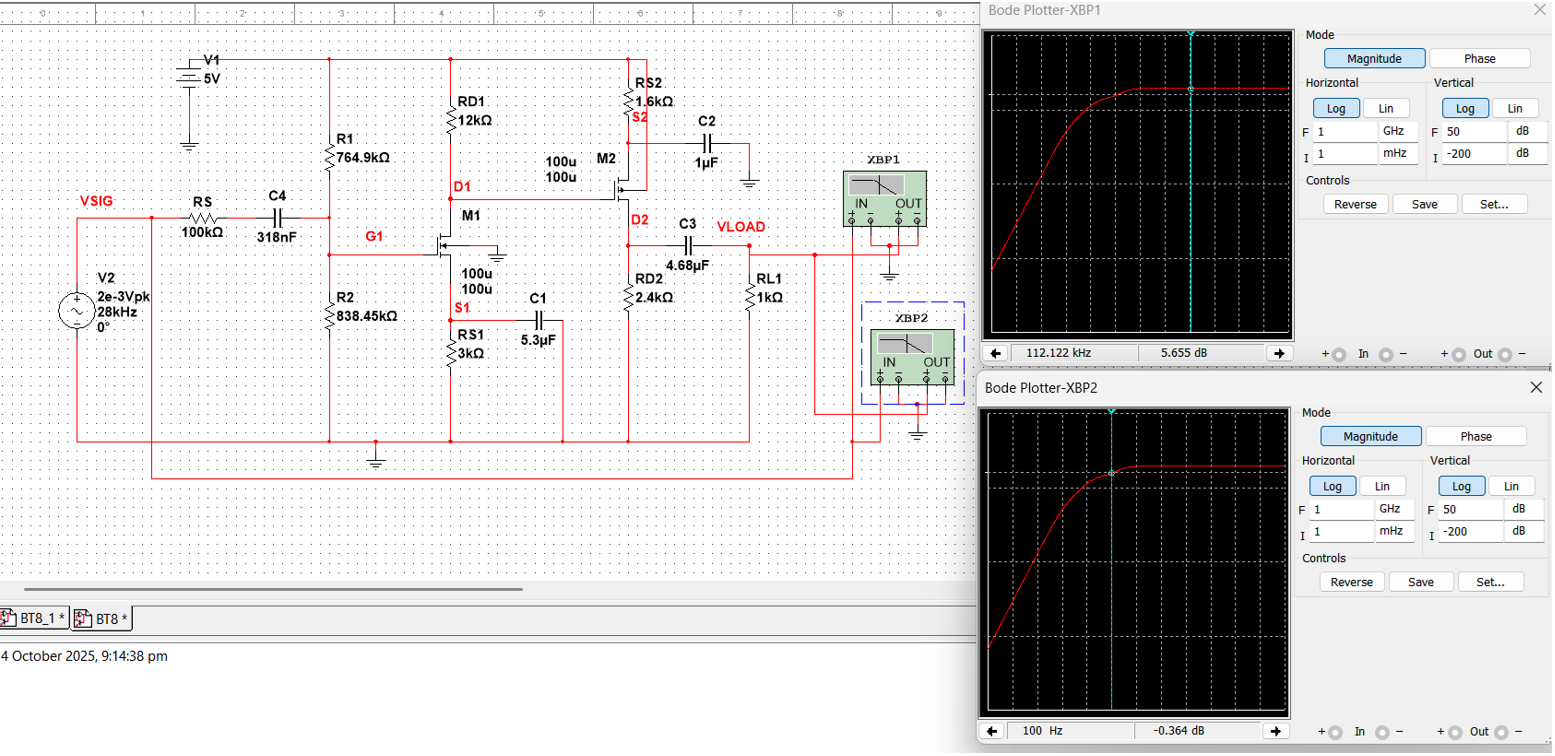
\includegraphics[width=.8\linewidth]{./my-chapters/my-images/Question8/d_ketqua1.png}
	\caption{Tại $f = 100 \textsf{Hz}$ $G_{v} = -0.364 db \neq 2.665 db$.}
\end{figure}

Để mạch có đúng tần số cắt tại $f = 100 \textsf{Hz}$ ta tiến hành sweep $C_{2}$ từ để tìm giá trị $C_{2}$ vì $f_{2}$ là cực chủ đạo.

\begin{figure}[H]
	\centering
	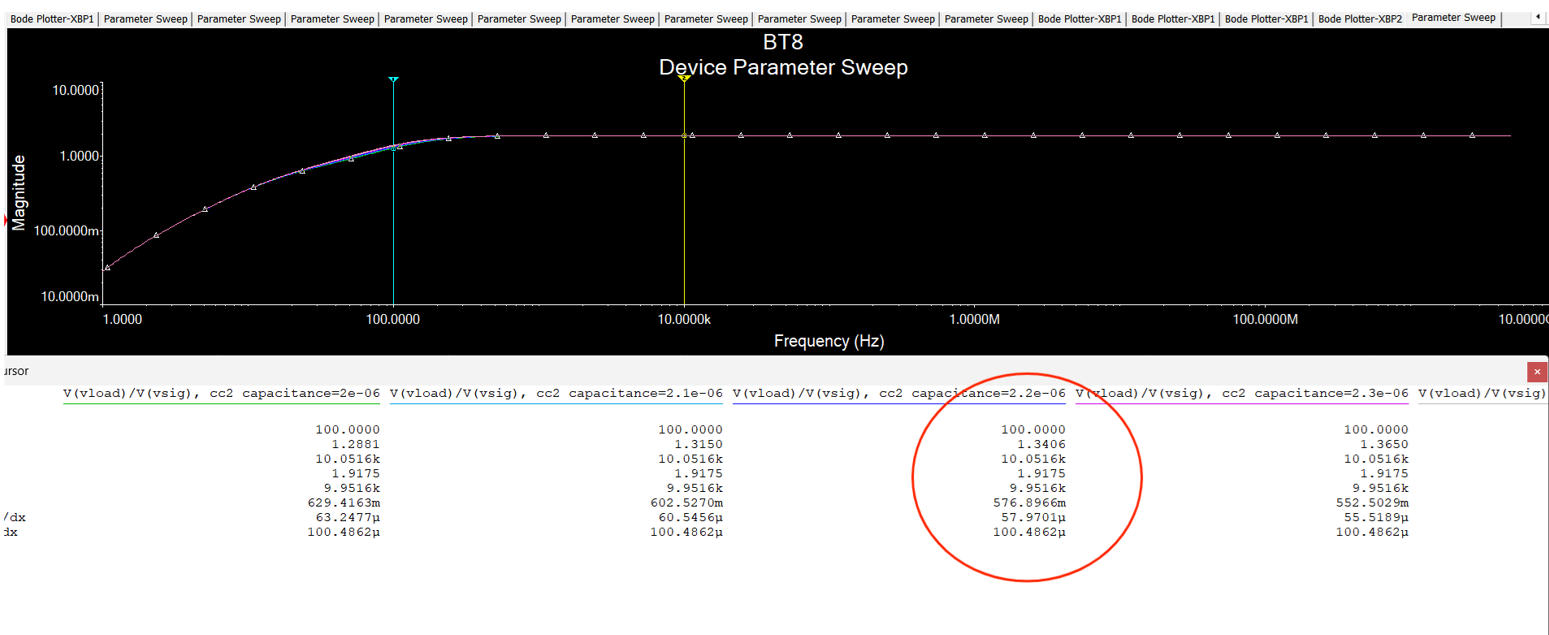
\includegraphics[width=.9\linewidth]{./my-chapters/my-images/Question8/d_ketqua2.png}
	\caption{Với $C_{2} = 2.2 \mu\textsf{F}$, tại $f = 100 \textsf{Hz}$ $G_{v} = 1.3406 \textsf{V/V} = 2.546db \approx 2.66db$.}
\end{figure}

\begin{figure}[H]
	\centering
	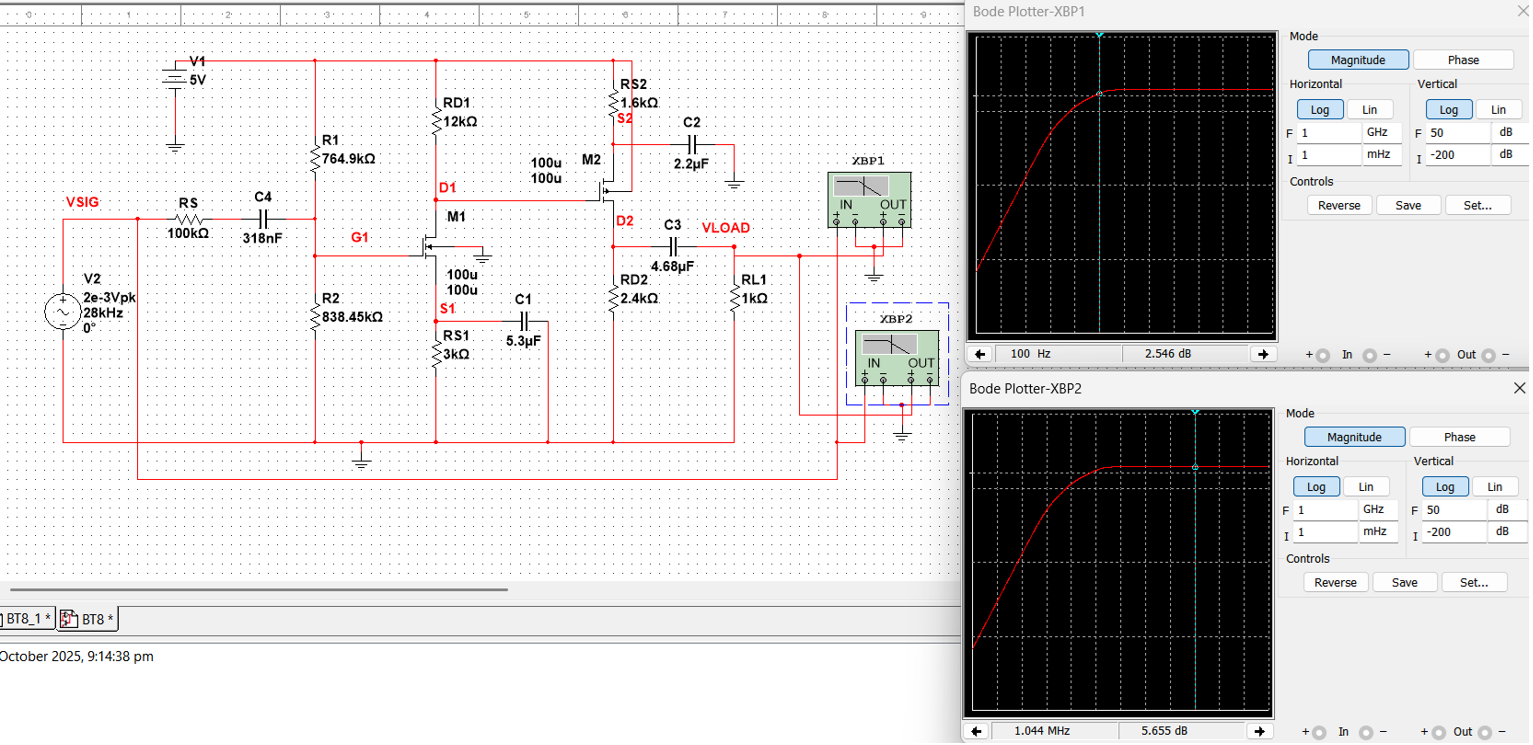
\includegraphics[width=.9\linewidth]{./my-chapters/my-images/Question8/d_ketqua3.png}
	\caption{Tại $f = 100 \textsf{hz}$ $G_{v} = 2.546 db \approx 2.665 db$.}
\end{figure}